\chapter[Desenvolvimento ]{Desenvolvimento}
Esta sessão tratará sobre como foi estabelecido o processo de verificação e
validação de um dado aterfato. Iremos abordar desde a escolha deste artefato até
a sua melhoria com o processos estabelecidos.
\section{Definição do Escopo}
\subsection{Disciplina }

A disciplina escolhida para experimentalmente ser analisada pela equipe é a disciplina de Análise e Design. Essa disciplina tem por finalidade converter a visão unilateral de requisitos em objetos mais palpáveis que trazem uma visão de design do sistema a ser criado. Contudo, trazer também uma visão mais sofisticada da arquitetura para o sistema.\cite{e01} 

Nessa disciplina de Análise e Design executam-se 6 microprocessos, onde no processo inicial verifica-se a viabilidade conforme o previsto, e avalia-se as tecnologias disponíveis para auxiliarem a produção. Com isso, o foco é direcionado ao desenvolvimento de uma arquitetura inicial para o sistema, e ai o enfoque passa a ser análise de comportamento e a criação de um conjunto inicial de elementos comportamentais.\cite{e02} 

\subsection{Produtos da Disciplina}
Com a execução do fluxo de trabalho os seguintes produtos são gerados na Tabela\cite{e03}  a seguir:

\begin{longtable}{||p{3cm}|p{5cm}|p{5cm}||}
\caption{Artefatos Gerados na Disciplina de Análise e Design}
\\ \hline
\textbf{Artefato} & \textbf{Finalidade} & \textbf{Adaptação (Opcional, Recomendada)} \\ \hline \hline                                                                                                                                                                                  
Modelo de análise (Classe de análise) (Necessário) & Um modelo de análise ajuda a compreender melhor os requisitos antes da tomada de decisões sobre design. Em sistemas complexos, ele pode ser mantido para fornecer uma visão geral conceitual do sistema.                                                                                                                                                                                                          & Opcional em muitos projetos, um Modelo de Design inicial é usado em lugar do Modelo de Análise.Em projetos que efetivamente criam um Modelo de Análise, normalmente é um artefato temporário que acaba se transformando em um modelo de design.                                                                                                                                   \\ \hline
Modelo de design (necessário)                      & É recomendável que a maioria dos sistemas (mesmo os menores) sejam projetados antes de serem implementados, a fim de evitar um retrabalho dispendioso decorrente de erros de design. Os modelos visuais permitem que o design seja facilmente comunicado. O uso de ferramentas de engenharia direta e de engenharia reversa pode assegurar a consistência com o modelo de implementação, além de poupar trabalho. & Recomendada para a maioria dos projetos.Em projetos menores, o uso de ferramentas automatizadas não é crítico, mas pode beneficiar a produtividade a longo prazo.                                                                                                                                                                                                                \\ \hline
Classe de design;Pacote de design                  & As classes e os pacotes são uma parte básica de qualquer design orientado a objetos. O design orientado a objetos é o método de design padrão utilizado na maior parte dos projetos.                                                                                                                                                                                                                              & Recomendada para a maioria dos projetos.Um dos principais problemas de adaptação é decidir quais estereótipos devem ser usados (isso poderá ser abordado no Guia de Design).                                                                                                                                                                                                     \\ \hline
Realização de caso de uso                          & Estabelece a conexão entre casos de uso e design.                                                                                                                                                                                                                                                                                                                                                                 & Recomendada para a maioria dos projetos.                                                                                                                                                                                                                                                                                                                                         \\ \hline
Interface                                          & Normalmente, as interfaces são usadas para definir um comportamento, sejam quais forem os componentes de baixa granularidade que assumam o comportamento.                                                                                                                                                                                                                                                         & Recomendada para a maioria dos projetos.O design baseado em componentes está se tornando uma abordagem de design padrão.                                                                                                                                                                                                                                                         \\ \hline
Subsistemas de design                              & Os subsistemas de design são usados para encapsular comportamento em um "pacote" que forneça interfaces. São usados para encapsular as interações de classes e/ou outros subsistemas.                                                                                                                                                                                                                             & Recomendada para a maioria dos projetos.Em geral, os subsistemas ajudam a elevar o nível de abstração do design. Eles tornam os sistemas mais fáceis.                                                                                                                                                                                                                            \\ \hline
Evento                                             & Pode ser útil para sistemas que respondem a muitos eventos externos.                                                                                                                                                                                                                                                                                                                                              & Recomendada para sistemas em tempo real.                                                                                                                                                                                                                                                                                                                                         \\ \hline
Protocolo                                          & Obrigatório para sistemas em tempo real.                                                                                                                                                                                                                                                                                                                                                                          & Recomendada para sistemas em tempo real.                                                                                                                                                                                                                                                                                                                                         \\ \hline
Sinal                                              & Pode ser útil para sistemas que necessitem de simultaneidade e sejam controlados por eventos. Obrigatório para sistemas em tempo real.                                                                                                                                                                                                                                                                            & Recomendada para sistemas em tempo real.Pode ser útil para sistemas que necessitem de simultaneidade e sejam controlados por eventos.                                                                                                                                                                                                                                            \\ \hline
Cápsula                                            & Destina-se a sistemas em tempo real, mas pode ser útil na modelagem e no design de qualquer sistema com alto grau de simultaneidade.                                                                                                                                                                                                                                                                              & Recomendada para sistemas em tempo real.                                                                                                                                                                                                                                                                                                                                         \\ \hline
Modelo de dados                                    & Usado para descrever a estrutura lógica e possivelmente física das informações persistentes.                                                                                                                                                                                                                                                                                                                      & Recomendada para projetos que utilizam um banco de dados.                                                                                                                                                                                                                                                                                                                        \\ \hline
Modelo de Implantação                              & Mostra a configuração de nós de processamento em tempo de execução e os vínculos de comunicação entre eles, assim como as instâncias de componentes e os objetos que neles residem.                                                                                                                                                                                                                               & Opcional.Muitos sistemas apresentam vários nós de processamento e, por isso, precisam utilizar o Modelo de Implantação. No entanto, ele pode ser abordado como uma seção do Documento de Arquitetura de Software, sem precisar existir como um artefato identificado separadamente.                                                                                              \\ \hline
Prova de Conceito Arquitetural                     & Usada para determinar se existe uma solução que satisfaça os requisitos significativos do ponto de vista arquitetural                                                                                                                                                                                                                                                                                             & Recomendada para a maioria dos projetos.Muitos projetos utilizam uma Prova de Conceito Arquitetural para determinar a viabilidade dos requisitos. Estas são algumas das muitas formas que ela pode assumir:uma lista de tecnologias conhecidas que pareça adequada à soluçãoum esboço de um modelo conceitual de uma soluçãouma simulação de uma soluçãoum protótipo executável. \\ \hline
Arquitetura de Referência                          & As Arquiteturas de Referência aceleram o desenvolvimento e reduzem os riscos reutilizando soluções já aprovadas.                                                                                                                                                                                                                                                                                                  & Recomendada para a maioria dos projetos.Se existir material de Arquitetura de Referência apropriado, ela pode acelerar o desenvolvimento e reduzir os riscos consideravelmente.                                                                                                                                                                                                  \\ \hline
Documento de Arquitetura de Software (SAD)         & O Documento de Arquitetura de Software é usado para fornecer uma ampla visão geral da arquitetura do sistema. Essa visão geral ajuda a compreender o sistema e a captar decisões arquiteturais importantes.                                                                                                                                                                                                       & Recomendada para a maioria dos projetos.Uma visão geral de alto nível da arquitetura do software é útil para todos os sistemas, exceto os menores. Normalmente, os sistemas complexos necessitam de um nível maior de detalhes e de mais visões que os projetos menores.                                                                                                         \\ \hline
\end{longtable}

\subsection{Definição do Escopo}
O Modelo de Dados foi definido como o produto gerado da disciplina que usaremos como objeto da verificação. Ele descreve uma representação lógica dos dados persistentes do sistema, alem de trazer em grande parte particularidades do comportamento do banco de dados.\cite{e04} 

Afim de direcionar a inspeção a seguinte ordem de inspeção e analise é proposta:

\begin{itemize}
\item Entidades
\item Atributos
\item Chaves
\item Relacionamentos
\item Coerência Nominal
\end{itemize}

\section{Definição do Processo de VeV}

\subsection{Escolha da Metodologia Estática}
Para a definição do processo de Verificação e Validação, utilizamos a revisão
estática Walkthrogth. Pois,  a equipe avaliadora é composta por técnicos no escopo
do artefato escolhido. Além disso, com este método estático, a equipe pode corroborar
junta a fim de estabelecer uma melhor verificação para o produto.

\subsection{Processo de VeV}
A modelagem de processos auxilia à nivelar o entendimento de todo o time sobre o processo a ser executado, além de manter 
um padrão nas atividades executadas\cite{romano} . Por isso, foi 
desenvolvido um processo de verificação e validação utilizando o método walkthrough. A imagem abaixo apresenta o processo 
modelado.

\begin{figure}[!h]
\centering
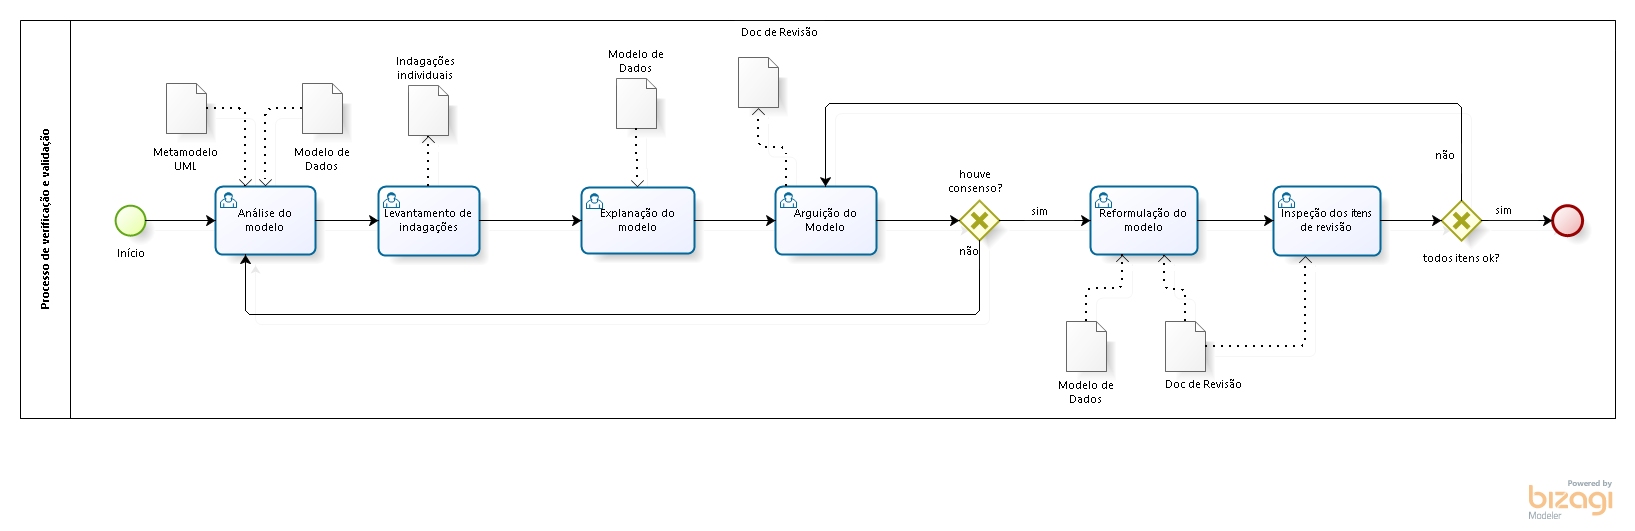
\includegraphics[scale=0.55, angle = 90]{figuras/Processo_vv_walkthrough}
\caption[Processo de Verificação e Validação Utilizado]{Processo de Verificação e Validação Utilizado\footnotemark}
\end{figure}
\FloatBarrier

A atividade "Análise do Modelo" é executada pela EVeV, e prevê uma análise do modelo de dados visando encontrar erros 
relacionados aos padrões UML e erros na modelagem do banco de dados. 

A atividade "Levantamento de Indagações" é executada pela EVeV, e prevê o levantamento e registros de questões e 
observações relacionadas ao modelo de dados. 

A atividade "Explanação do modelo" é executada pela Dona do Produto, e prevê uma explicação do modelo de dados visando 
proporcionar um entendimento geral do modelo.

A atividade "Arguição do Modelo" é executada pela Dona do Produto e pela EVeV, e prevê uma apresentação dos erros e 
dúvidas por parte da equipe de EVeV e resposta por parte da Dona do Produto.

A atividade "Reformulação do Modelo" é executada pela Dona do Produto, visando a adequação com os itens do Documento de 
Revisão.

A atividade "Inspeção dos itens de revisão" é executada pela equipe de EVeV, e prevê uma verificação se todos os itens 
propostos no Documento de Revisão foram atendidos.

Por meio desse processo, o time conseguiu realizar com sucesso o processo de verificação e validação.	


\subsection{Produtos de Auxílio}
Para desenvolver os trabalhos da revisão estática, são necessários alguns artefatos
de auxílio. Destes, teremos:

\begin{itemize}
\item Metamodelo UML - Documento de embasamento para o estabelecimento da sintaxe
de metamodelo de dados
\item Indagações Individuais - Pontos que cada avaliador do documento julgou como
importante para a melhoria do artefato
\item Checklist - Documento de Revisão, criado para ponderar os pontos acordados
entre as partes para a refatoração do trabalho.
\end{itemize}

\subsection{Infraestrutura Utilizada}
Quanto aos esquipamentos físicos e softwares utilizados para desenvolver a Verificação
e validação do produto, tivemos:

\begin{itemize}
  \item Quatro Notebooks - Ferramentas para desenvolvimento
  \item Software de Modelagem de Dados - Utilizada para representar o modelo de
  banco de dados da aplicação
  \item Software de Modelagem de Processos (Bizagi) - Responsável pelo desenho do
  processo adotado pelo time.
\end{itemize}

\subsection{Participantes}
Para verificar e validar o artefato escolhido, teremos duas equipes. A primeira é
constituída pelo Dono do Produto, que conhece o domínio e que está desenvolvendo
a modelagem dos dados. A segunda trata-se da EVeV, que avaliará o documento
pelo método estático do Walkthrogth.

\subsection{Resultados Esperados}
Após obtermos todo o feedback e refatoração a partir dos pontos levantados no
Documento de Revisão, espera-se uma modelagem de dados mais robusta e que proporcione
maior satisfação para o cliente final.
